\documentclass{report}

%%%%%%%%%%%%%%%%%%%%%%%%%%%%%%%%%
% PACKAGE IMPORTS
%%%%%%%%%%%%%%%%%%%%%%%%%%%%%%%%%


\usepackage[tmargin=2cm,rmargin=1in,lmargin=1in,margin=0.85in,bmargin=2cm,footskip=.2in]{geometry}
\usepackage{amsmath,amsfonts,amsthm,amssymb,mathtools}
\usepackage[varbb]{newpxmath}
\usepackage{xfrac}
\usepackage[makeroom]{cancel}
\usepackage{mathtools}
\usepackage{bookmark}
\usepackage{enumitem}
\usepackage{hyperref,theoremref}
\hypersetup{
	pdftitle={Assignment},
	colorlinks=true, linkcolor=doc!90,
	bookmarksnumbered=true,
	bookmarksopen=true
}
\usepackage[most,many,breakable]{tcolorbox}
\usepackage{xcolor}
\usepackage{varwidth}
\usepackage{varwidth}
\usepackage{etoolbox}
%\usepackage{authblk}
\usepackage{nameref}
\usepackage{multicol,array}
\usepackage{tikz-cd}
\usepackage[ruled,vlined,linesnumbered]{algorithm2e}
\usepackage{comment} % enables the use of multi-line comments (\ifx \fi) 
\usepackage{import}
\usepackage{xifthen}
\usepackage{pdfpages}
\usepackage{transparent}

\newcommand\mycommfont[1]{\footnotesize\ttfamily\textcolor{blue}{#1}}
\SetCommentSty{mycommfont}
\newcommand{\incfig}[1]{%
    \def\svgwidth{\columnwidth}
    \import{./figures/}{#1.pdf_tex}
}

\usepackage{tikzsymbols}
\renewcommand\qedsymbol{$\Laughey$}


%\usepackage{import}
%\usepackage{xifthen}
%\usepackage{pdfpages}
%\usepackage{transparent}


%%%%%%%%%%%%%%%%%%%%%%%%%%%%%%
% SELF MADE COLORS
%%%%%%%%%%%%%%%%%%%%%%%%%%%%%%



\definecolor{myg}{RGB}{56, 140, 70}
\definecolor{myb}{RGB}{45, 111, 177}
\definecolor{myr}{RGB}{199, 68, 64}
\definecolor{mytheorembg}{HTML}{F2F2F9}
\definecolor{mytheoremfr}{HTML}{00007B}
\definecolor{mylenmabg}{HTML}{FFFAF8}
\definecolor{mylenmafr}{HTML}{983b0f}
\definecolor{mypropbg}{HTML}{f2fbfc}
\definecolor{mypropfr}{HTML}{191971}
\definecolor{myexamplebg}{HTML}{F2FBF8}
\definecolor{myexamplefr}{HTML}{88D6D1}
\definecolor{myexampleti}{HTML}{2A7F7F}
\definecolor{mydefinitbg}{HTML}{E5E5FF}
\definecolor{mydefinitfr}{HTML}{3F3FA3}
\definecolor{notesgreen}{RGB}{0,162,0}
\definecolor{myp}{RGB}{197, 92, 212}
\definecolor{mygr}{HTML}{2C3338}
\definecolor{myred}{RGB}{127,0,0}
\definecolor{myyellow}{RGB}{169,121,69}
\definecolor{myexercisebg}{HTML}{F2FBF8}
\definecolor{myexercisefg}{HTML}{88D6D1}


%%%%%%%%%%%%%%%%%%%%%%%%%%%%
% TCOLORBOX SETUPS
%%%%%%%%%%%%%%%%%%%%%%%%%%%%

\setlength{\parindent}{1cm}
%================================
% THEOREM BOX
%================================

\tcbuselibrary{theorems,skins,hooks}
\newtcbtheorem[number within=section]{Theorem}{Theorem}
{%
	enhanced,
	breakable,
	colback = mytheorembg,
	frame hidden,
	boxrule = 0sp,
	borderline west = {2pt}{0pt}{mytheoremfr},
	sharp corners,
	detach title,
	before upper = \tcbtitle\par\smallskip,
	coltitle = mytheoremfr,
	fonttitle = \bfseries\sffamily,
	description font = \mdseries,
	separator sign none,
	segmentation style={solid, mytheoremfr},
}
{th}

\tcbuselibrary{theorems,skins,hooks}
\newtcbtheorem[number within=chapter]{theorem}{Theorem}
{%
	enhanced,
	breakable,
	colback = mytheorembg,
	frame hidden,
	boxrule = 0sp,
	borderline west = {2pt}{0pt}{mytheoremfr},
	sharp corners,
	detach title,
	before upper = \tcbtitle\par\smallskip,
	coltitle = mytheoremfr,
	fonttitle = \bfseries\sffamily,
	description font = \mdseries,
	separator sign none,
	segmentation style={solid, mytheoremfr},
}
{th}


\tcbuselibrary{theorems,skins,hooks}
\newtcolorbox{Theoremcon}
{%
	enhanced
	,breakable
	,colback = mytheorembg
	,frame hidden
	,boxrule = 0sp
	,borderline west = {2pt}{0pt}{mytheoremfr}
	,sharp corners
	,description font = \mdseries
	,separator sign none
}

%================================
% Corollery
%================================
\tcbuselibrary{theorems,skins,hooks}
\newtcbtheorem[number within=section]{Corollary}{Corollary}
{%
	enhanced
	,breakable
	,colback = myp!10
	,frame hidden
	,boxrule = 0sp
	,borderline west = {2pt}{0pt}{myp!85!black}
	,sharp corners
	,detach title
	,before upper = \tcbtitle\par\smallskip
	,coltitle = myp!85!black
	,fonttitle = \bfseries\sffamily
	,description font = \mdseries
	,separator sign none
	,segmentation style={solid, myp!85!black}
}
{th}
\tcbuselibrary{theorems,skins,hooks}
\newtcbtheorem[number within=chapter]{corollary}{Corollary}
{%
	enhanced
	,breakable
	,colback = myp!10
	,frame hidden
	,boxrule = 0sp
	,borderline west = {2pt}{0pt}{myp!85!black}
	,sharp corners
	,detach title
	,before upper = \tcbtitle\par\smallskip
	,coltitle = myp!85!black
	,fonttitle = \bfseries\sffamily
	,description font = \mdseries
	,separator sign none
	,segmentation style={solid, myp!85!black}
}
{th}


%================================
% LENMA
%================================

\tcbuselibrary{theorems,skins,hooks}
\newtcbtheorem[number within=section]{Lenma}{Lenma}
{%
	enhanced,
	breakable,
	colback = mylenmabg,
	frame hidden,
	boxrule = 0sp,
	borderline west = {2pt}{0pt}{mylenmafr},
	sharp corners,
	detach title,
	before upper = \tcbtitle\par\smallskip,
	coltitle = mylenmafr,
	fonttitle = \bfseries\sffamily,
	description font = \mdseries,
	separator sign none,
	segmentation style={solid, mylenmafr},
}
{th}

\tcbuselibrary{theorems,skins,hooks}
\newtcbtheorem[number within=chapter]{lenma}{Lenma}
{%
	enhanced,
	breakable,
	colback = mylenmabg,
	frame hidden,
	boxrule = 0sp,
	borderline west = {2pt}{0pt}{mylenmafr},
	sharp corners,
	detach title,
	before upper = \tcbtitle\par\smallskip,
	coltitle = mylenmafr,
	fonttitle = \bfseries\sffamily,
	description font = \mdseries,
	separator sign none,
	segmentation style={solid, mylenmafr},
}
{th}


%================================
% PROPOSITION
%================================

\tcbuselibrary{theorems,skins,hooks}
\newtcbtheorem[number within=section]{Prop}{Proposition}
{%
	enhanced,
	breakable,
	colback = mypropbg,
	frame hidden,
	boxrule = 0sp,
	borderline west = {2pt}{0pt}{mypropfr},
	sharp corners,
	detach title,
	before upper = \tcbtitle\par\smallskip,
	coltitle = mypropfr,
	fonttitle = \bfseries\sffamily,
	description font = \mdseries,
	separator sign none,
	segmentation style={solid, mypropfr},
}
{th}

\tcbuselibrary{theorems,skins,hooks}
\newtcbtheorem[number within=chapter]{prop}{Proposition}
{%
	enhanced,
	breakable,
	colback = mypropbg,
	frame hidden,
	boxrule = 0sp,
	borderline west = {2pt}{0pt}{mypropfr},
	sharp corners,
	detach title,
	before upper = \tcbtitle\par\smallskip,
	coltitle = mypropfr,
	fonttitle = \bfseries\sffamily,
	description font = \mdseries,
	separator sign none,
	segmentation style={solid, mypropfr},
}
{th}


%================================
% CLAIM
%================================

\tcbuselibrary{theorems,skins,hooks}
\newtcbtheorem[number within=section]{claim}{Claim}
{%
	enhanced
	,breakable
	,colback = myg!10
	,frame hidden
	,boxrule = 0sp
	,borderline west = {2pt}{0pt}{myg}
	,sharp corners
	,detach title
	,before upper = \tcbtitle\par\smallskip
	,coltitle = myg!85!black
	,fonttitle = \bfseries\sffamily
	,description font = \mdseries
	,separator sign none
	,segmentation style={solid, myg!85!black}
}
{th}



%================================
% Exercise
%================================

\tcbuselibrary{theorems,skins,hooks}
\newtcbtheorem[number within=section]{Exercise}{Exercise}
{%
	enhanced,
	breakable,
	colback = myexercisebg,
	frame hidden,
	boxrule = 0sp,
	borderline west = {2pt}{0pt}{myexercisefg},
	sharp corners,
	detach title,
	before upper = \tcbtitle\par\smallskip,
	coltitle = myexercisefg,
	fonttitle = \bfseries\sffamily,
	description font = \mdseries,
	separator sign none,
	segmentation style={solid, myexercisefg},
}
{th}

\tcbuselibrary{theorems,skins,hooks}
\newtcbtheorem[number within=chapter]{exercise}{Exercise}
{%
	enhanced,
	breakable,
	colback = myexercisebg,
	frame hidden,
	boxrule = 0sp,
	borderline west = {2pt}{0pt}{myexercisefg},
	sharp corners,
	detach title,
	before upper = \tcbtitle\par\smallskip,
	coltitle = myexercisefg,
	fonttitle = \bfseries\sffamily,
	description font = \mdseries,
	separator sign none,
	segmentation style={solid, myexercisefg},
}
{th}

%================================
% EXAMPLE BOX
%================================

\newtcbtheorem[number within=section]{Example}{Example}
{%
	colback = myexamplebg
	,breakable
	,colframe = myexamplefr
	,coltitle = myexampleti
	,boxrule = 1pt
	,sharp corners
	,detach title
	,before upper=\tcbtitle\par\smallskip
	,fonttitle = \bfseries
	,description font = \mdseries
	,separator sign none
	,description delimiters parenthesis
}
{ex}

\newtcbtheorem[number within=chapter]{example}{Example}
{%
	colback = myexamplebg
	,breakable
	,colframe = myexamplefr
	,coltitle = myexampleti
	,boxrule = 1pt
	,sharp corners
	,detach title
	,before upper=\tcbtitle\par\smallskip
	,fonttitle = \bfseries
	,description font = \mdseries
	,separator sign none
	,description delimiters parenthesis
}
{ex}

%================================
% DEFINITION BOX
%================================

\newtcbtheorem[number within=section]{Definition}{Definition}{enhanced,
	before skip=2mm,after skip=2mm, colback=red!5,colframe=red!80!black,boxrule=0.5mm,
	attach boxed title to top left={xshift=1cm,yshift*=1mm-\tcboxedtitleheight}, varwidth boxed title*=-3cm,
	boxed title style={frame code={
					\path[fill=tcbcolback]
					([yshift=-1mm,xshift=-1mm]frame.north west)
					arc[start angle=0,end angle=180,radius=1mm]
					([yshift=-1mm,xshift=1mm]frame.north east)
					arc[start angle=180,end angle=0,radius=1mm];
					\path[left color=tcbcolback!60!black,right color=tcbcolback!60!black,
						middle color=tcbcolback!80!black]
					([xshift=-2mm]frame.north west) -- ([xshift=2mm]frame.north east)
					[rounded corners=1mm]-- ([xshift=1mm,yshift=-1mm]frame.north east)
					-- (frame.south east) -- (frame.south west)
					-- ([xshift=-1mm,yshift=-1mm]frame.north west)
					[sharp corners]-- cycle;
				},interior engine=empty,
		},
	fonttitle=\bfseries,
	title={#2},#1}{def}
\newtcbtheorem[number within=chapter]{definition}{Definition}{enhanced,
	before skip=2mm,after skip=2mm, colback=red!5,colframe=red!80!black,boxrule=0.5mm,
	attach boxed title to top left={xshift=1cm,yshift*=1mm-\tcboxedtitleheight}, varwidth boxed title*=-3cm,
	boxed title style={frame code={
					\path[fill=tcbcolback]
					([yshift=-1mm,xshift=-1mm]frame.north west)
					arc[start angle=0,end angle=180,radius=1mm]
					([yshift=-1mm,xshift=1mm]frame.north east)
					arc[start angle=180,end angle=0,radius=1mm];
					\path[left color=tcbcolback!60!black,right color=tcbcolback!60!black,
						middle color=tcbcolback!80!black]
					([xshift=-2mm]frame.north west) -- ([xshift=2mm]frame.north east)
					[rounded corners=1mm]-- ([xshift=1mm,yshift=-1mm]frame.north east)
					-- (frame.south east) -- (frame.south west)
					-- ([xshift=-1mm,yshift=-1mm]frame.north west)
					[sharp corners]-- cycle;
				},interior engine=empty,
		},
	fonttitle=\bfseries,
	title={#2},#1}{def}



%================================
% Solution BOX
%================================

\makeatletter
\newtcbtheorem{question}{Question}{enhanced,
	breakable,
	colback=white,
	colframe=myb!80!black,
	attach boxed title to top left={yshift*=-\tcboxedtitleheight},
	fonttitle=\bfseries,
	title={#2},
	boxed title size=title,
	boxed title style={%
			sharp corners,
			rounded corners=northwest,
			colback=tcbcolframe,
			boxrule=0pt,
		},
	underlay boxed title={%
			\path[fill=tcbcolframe] (title.south west)--(title.south east)
			to[out=0, in=180] ([xshift=5mm]title.east)--
			(title.center-|frame.east)
			[rounded corners=\kvtcb@arc] |-
			(frame.north) -| cycle;
		},
	#1
}{def}
\makeatother

%================================
% SOLUTION BOX
%================================

\makeatletter
\newtcolorbox{solution}{enhanced,
	breakable,
	colback=white,
	colframe=myg!80!black,
	attach boxed title to top left={yshift*=-\tcboxedtitleheight},
	title=Solution,
	boxed title size=title,
	boxed title style={%
			sharp corners,
			rounded corners=northwest,
			colback=tcbcolframe,
			boxrule=0pt,
		},
	underlay boxed title={%
			\path[fill=tcbcolframe] (title.south west)--(title.south east)
			to[out=0, in=180] ([xshift=5mm]title.east)--
			(title.center-|frame.east)
			[rounded corners=\kvtcb@arc] |-
			(frame.north) -| cycle;
		},
}
\makeatother

%================================
% Question BOX
%================================

\makeatletter
\newtcbtheorem{qstion}{Question}{enhanced,
	breakable,
	colback=white,
	colframe=mygr,
	attach boxed title to top left={yshift*=-\tcboxedtitleheight},
	fonttitle=\bfseries,
	title={#2},
	boxed title size=title,
	boxed title style={%
			sharp corners,
			rounded corners=northwest,
			colback=tcbcolframe,
			boxrule=0pt,
		},
	underlay boxed title={%
			\path[fill=tcbcolframe] (title.south west)--(title.south east)
			to[out=0, in=180] ([xshift=5mm]title.east)--
			(title.center-|frame.east)
			[rounded corners=\kvtcb@arc] |-
			(frame.north) -| cycle;
		},
	#1
}{def}
\makeatother

\newtcbtheorem[number within=chapter]{wconc}{Wrong Concept}{
	breakable,
	enhanced,
	colback=white,
	colframe=myr,
	arc=0pt,
	outer arc=0pt,
	fonttitle=\bfseries\sffamily\large,
	colbacktitle=myr,
	attach boxed title to top left={},
	boxed title style={
			enhanced,
			skin=enhancedfirst jigsaw,
			arc=3pt,
			bottom=0pt,
			interior style={fill=myr}
		},
	#1
}{def}



%================================
% NOTE BOX
%================================

\usetikzlibrary{arrows,calc,shadows.blur}
\tcbuselibrary{skins}
\newtcolorbox{note}[1][]{%
	enhanced jigsaw,
	colback=gray!20!white,%
	colframe=gray!80!black,
	size=small,
	boxrule=1pt,
	title=\textbf{Note:-},
	halign title=flush center,
	coltitle=black,
	breakable,
	drop shadow=black!50!white,
	attach boxed title to top left={xshift=1cm,yshift=-\tcboxedtitleheight/2,yshifttext=-\tcboxedtitleheight/2},
	minipage boxed title=1.5cm,
	boxed title style={%
			colback=white,
			size=fbox,
			boxrule=1pt,
			boxsep=2pt,
			underlay={%
					\coordinate (dotA) at ($(interior.west) + (-0.5pt,0)$);
					\coordinate (dotB) at ($(interior.east) + (0.5pt,0)$);
					\begin{scope}
						\clip (interior.north west) rectangle ([xshift=3ex]interior.east);
						\filldraw [white, blur shadow={shadow opacity=60, shadow yshift=-.75ex}, rounded corners=2pt] (interior.north west) rectangle (interior.south east);
					\end{scope}
					\begin{scope}[gray!80!black]
						\fill (dotA) circle (2pt);
						\fill (dotB) circle (2pt);
					\end{scope}
				},
		},
	#1,
}

%%%%%%%%%%%%%%%%%%%%%%%%%%%%%%
% SELF MADE COMMANDS
%%%%%%%%%%%%%%%%%%%%%%%%%%%%%%


\newcommand{\thm}[2]{\begin{Theorem}{#1}{}#2\end{Theorem}}
\newcommand{\cor}[2]{\begin{Corollary}{#1}{}#2\end{Corollary}}
\newcommand{\mlenma}[2]{\begin{Lenma}{#1}{}#2\end{Lenma}}
\newcommand{\mprop}[2]{\begin{Prop}{#1}{}#2\end{Prop}}
\newcommand{\clm}[3]{\begin{claim}{#1}{#2}#3\end{claim}}
\newcommand{\wc}[2]{\begin{wconc}{#1}{}\setlength{\parindent}{1cm}#2\end{wconc}}
\newcommand{\thmcon}[1]{\begin{Theoremcon}{#1}\end{Theoremcon}}
\newcommand{\ex}[2]{\begin{Example}{#1}{}#2\end{Example}}
\newcommand{\dfn}[2]{\begin{Definition}[colbacktitle=red!75!black]{#1}{}#2\end{Definition}}
\newcommand{\dfnc}[2]{\begin{definition}[colbacktitle=red!75!black]{#1}{}#2\end{definition}}
\newcommand{\qs}[2]{\begin{question}{#1}{}#2\end{question}}
\newcommand{\pf}[2]{\begin{myproof}[#1]#2\end{myproof}}
\newcommand{\nt}[1]{\begin{note}#1\end{note}}

\newcommand*\circled[1]{\tikz[baseline=(char.base)]{
		\node[shape=circle,draw,inner sep=1pt] (char) {#1};}}
\newcommand\getcurrentref[1]{%
	\ifnumequal{\value{#1}}{0}
	{??}
	{\the\value{#1}}%
}
\newcommand{\getCurrentSectionNumber}{\getcurrentref{section}}
\newenvironment{myproof}[1][\proofname]{%
	\proof[\bfseries #1: ]%
}{\endproof}

\newcommand{\mclm}[2]{\begin{myclaim}[#1]#2\end{myclaim}}
\newenvironment{myclaim}[1][\claimname]{\proof[\bfseries #1: ]}{}

\newcounter{mylabelcounter}

\makeatletter
\newcommand{\setword}[2]{%
	\phantomsection
	#1\def\@currentlabel{\unexpanded{#1}}\label{#2}%
}
\makeatother




\tikzset{
	symbol/.style={
			draw=none,
			every to/.append style={
					edge node={node [sloped, allow upside down, auto=false]{$#1$}}}
		}
}


% deliminators
\DeclarePairedDelimiter{\abs}{\lvert}{\rvert}
\DeclarePairedDelimiter{\norm}{\lVert}{\rVert}

\DeclarePairedDelimiter{\ceil}{\lceil}{\rceil}
\DeclarePairedDelimiter{\floor}{\lfloor}{\rfloor}
\DeclarePairedDelimiter{\round}{\lfloor}{\rceil}

\newsavebox\diffdbox
\newcommand{\slantedromand}{{\mathpalette\makesl{d}}}
\newcommand{\makesl}[2]{%
\begingroup
\sbox{\diffdbox}{$\mathsurround=0pt#1\mathrm{#2}$}%
\pdfsave
\pdfsetmatrix{1 0 0.2 1}%
\rlap{\usebox{\diffdbox}}%
\pdfrestore
\hskip\wd\diffdbox
\endgroup
}
\newcommand{\dd}[1][]{\ensuremath{\mathop{}\!\ifstrempty{#1}{%
\slantedromand\@ifnextchar^{\hspace{0.2ex}}{\hspace{0.1ex}}}%
{\slantedromand\hspace{0.2ex}^{#1}}}}
\ProvideDocumentCommand\dv{o m g}{%
  \ensuremath{%
    \IfValueTF{#3}{%
      \IfNoValueTF{#1}{%
        \frac{\dd #2}{\dd #3}%
      }{%
        \frac{\dd^{#1} #2}{\dd #3^{#1}}%
      }%
    }{%
      \IfNoValueTF{#1}{%
        \frac{\dd}{\dd #2}%
      }{%
        \frac{\dd^{#1}}{\dd #2^{#1}}%
      }%
    }%
  }%
}
\providecommand*{\pdv}[3][]{\frac{\partial^{#1}#2}{\partial#3^{#1}}}
%  - others
\DeclareMathOperator{\Lap}{\mathcal{L}}
\DeclareMathOperator{\Var}{Var} % varience
\DeclareMathOperator{\Cov}{Cov} % covarience
\DeclareMathOperator{\E}{E} % expected

% Since the amsthm package isn't loaded

% I prefer the slanted \leq
\let\oldleq\leq % save them in case they're every wanted
\let\oldgeq\geq
\renewcommand{\leq}{\leqslant}
\renewcommand{\geq}{\geqslant}

% % redefine matrix env to allow for alignment, use r as default
% \renewcommand*\env@matrix[1][r]{\hskip -\arraycolsep
%     \let\@ifnextchar\new@ifnextchar
%     \array{*\c@MaxMatrixCols #1}}


%\usepackage{framed}
%\usepackage{titletoc}
%\usepackage{etoolbox}
%\usepackage{lmodern}


%\patchcmd{\tableofcontents}{\contentsname}{\sffamily\contentsname}{}{}

%\renewenvironment{leftbar}
%{\def\FrameCommand{\hspace{6em}%
%		{\color{myyellow}\vrule width 2pt depth 6pt}\hspace{1em}}%
%	\MakeFramed{\parshape 1 0cm \dimexpr\textwidth-6em\relax\FrameRestore}\vskip2pt%
%}
%{\endMakeFramed}

%\titlecontents{chapter}
%[0em]{\vspace*{2\baselineskip}}
%{\parbox{4.5em}{%
%		\hfill\Huge\sffamily\bfseries\color{myred}\thecontentspage}%
%	\vspace*{-2.3\baselineskip}\leftbar\textsc{\small\chaptername~\thecontentslabel}\\\sffamily}
%{}{\endleftbar}
%\titlecontents{section}
%[8.4em]
%{\sffamily\contentslabel{3em}}{}{}
%{\hspace{0.5em}\nobreak\itshape\color{myred}\contentspage}
%\titlecontents{subsection}
%[8.4em]
%{\sffamily\contentslabel{3em}}{}{}  
%{\hspace{0.5em}\nobreak\itshape\color{myred}\contentspage}



%%%%%%%%%%%%%%%%%%%%%%%%%%%%%%%%%%%%%%%%%%%
% TABLE OF CONTENTS
%%%%%%%%%%%%%%%%%%%%%%%%%%%%%%%%%%%%%%%%%%%

\usepackage{tikz}
\definecolor{doc}{RGB}{0,60,110}
\usepackage{titletoc}
\contentsmargin{0cm}
\titlecontents{chapter}[3.7pc]
{\addvspace{30pt}%
	\begin{tikzpicture}[remember picture, overlay]%
		\draw[fill=doc!60,draw=doc!60] (-7,-.1) rectangle (-0.9,.5);%
		\pgftext[left,x=-3.5cm,y=0.2cm]{\color{white}\Large\sc\bfseries Chapter\ \thecontentslabel};%
	\end{tikzpicture}\color{doc!60}\large\sc\bfseries}%
{}
{}
{\;\titlerule\;\large\sc\bfseries Page \thecontentspage
	\begin{tikzpicture}[remember picture, overlay]
		\draw[fill=doc!60,draw=doc!60] (2pt,0) rectangle (4,0.1pt);
	\end{tikzpicture}}%
\titlecontents{section}[3.7pc]
{\addvspace{2pt}}
{\contentslabel[\thecontentslabel]{2pc}}
{}
{\hfill\small \thecontentspage}
[]
\titlecontents*{subsection}[3.7pc]
{\addvspace{-1pt}\small}
{}
{}
{\ --- \small\thecontentspage}
[ \textbullet\ ][]

\makeatletter
\renewcommand{\tableofcontents}{%
	\chapter*{%
	  \vspace*{-20\p@}%
	  \begin{tikzpicture}[remember picture, overlay]%
		  \pgftext[right,x=15cm,y=0.2cm]{\color{doc!60}\Huge\sc\bfseries \contentsname};%
		  \draw[fill=doc!60,draw=doc!60] (13,-.75) rectangle (20,1);%
		  \clip (13,-.75) rectangle (20,1);
		  \pgftext[right,x=15cm,y=0.2cm]{\color{white}\Huge\sc\bfseries \contentsname};%
	  \end{tikzpicture}}%
	\@starttoc{toc}}
\makeatother


%From M275 "Topology" at SJSU
\newcommand{\id}{\mathrm{id}}
\newcommand{\taking}[1]{\xrightarrow{#1}}
\newcommand{\inv}{^{-1}}

%From M170 "Introduction to Graph Theory" at SJSU
\DeclareMathOperator{\diam}{diam}
\DeclareMathOperator{\ord}{ord}
\newcommand{\defeq}{\overset{\mathrm{def}}{=}}

%From the USAMO .tex files
\newcommand{\ts}{\textsuperscript}
\newcommand{\dg}{^\circ}
\newcommand{\ii}{\item}

% % From Math 55 and Math 145 at Harvard
% \newenvironment{subproof}[1][Proof]{%
% \begin{proof}[#1] \renewcommand{\qedsymbol}{$\blacksquare$}}%
% {\end{proof}}

\newcommand{\liff}{\leftrightarrow}
\newcommand{\lthen}{\rightarrow}
\newcommand{\opname}{\operatorname}
\newcommand{\surjto}{\twoheadrightarrow}
\newcommand{\injto}{\hookrightarrow}
\newcommand{\On}{\mathrm{On}} % ordinals
\DeclareMathOperator{\img}{im} % Image
\DeclareMathOperator{\Img}{Im} % Image
\DeclareMathOperator{\coker}{coker} % Cokernel
\DeclareMathOperator{\Coker}{Coker} % Cokernel
\DeclareMathOperator{\Ker}{Ker} % Kernel
\DeclareMathOperator{\rank}{rank}
\DeclareMathOperator{\Spec}{Spec} % spectrum
\DeclareMathOperator{\Tr}{Tr} % trace
\DeclareMathOperator{\pr}{pr} % projection
\DeclareMathOperator{\ext}{ext} % extension
\DeclareMathOperator{\pred}{pred} % predecessor
\DeclareMathOperator{\dom}{dom} % domain
\DeclareMathOperator{\ran}{ran} % range
\DeclareMathOperator{\Hom}{Hom} % homomorphism
\DeclareMathOperator{\Mor}{Mor} % morphisms
\DeclareMathOperator{\End}{End} % endomorphism

\newcommand{\eps}{\epsilon}
\newcommand{\veps}{\varepsilon}
\newcommand{\ol}{\overline}
\newcommand{\ul}{\underline}
\newcommand{\wt}{\widetilde}
\newcommand{\wh}{\widehat}
\newcommand{\vocab}[1]{\textbf{\color{blue} #1}}
\providecommand{\half}{\frac{1}{2}}
\newcommand{\dang}{\measuredangle} %% Directed angle
\newcommand{\ray}[1]{\overrightarrow{#1}}
\newcommand{\seg}[1]{\overline{#1}}
\newcommand{\arc}[1]{\wideparen{#1}}
\DeclareMathOperator{\cis}{cis}
\DeclareMathOperator*{\lcm}{lcm}
\DeclareMathOperator*{\argmin}{arg min}
\DeclareMathOperator*{\argmax}{arg max}
\newcommand{\cycsum}{\sum_{\mathrm{cyc}}}
\newcommand{\symsum}{\sum_{\mathrm{sym}}}
\newcommand{\cycprod}{\prod_{\mathrm{cyc}}}
\newcommand{\symprod}{\prod_{\mathrm{sym}}}
\newcommand{\Qed}{\begin{flushright}\qed\end{flushright}}
\newcommand{\parinn}{\setlength{\parindent}{1cm}}
\newcommand{\parinf}{\setlength{\parindent}{0cm}}
% \newcommand{\norm}{\|\cdot\|}
\newcommand{\inorm}{\norm_{\infty}}
\newcommand{\opensets}{\{V_{\alpha}\}_{\alpha\in I}}
\newcommand{\oset}{V_{\alpha}}
\newcommand{\opset}[1]{V_{\alpha_{#1}}}
\newcommand{\lub}{\text{lub}}
\newcommand{\del}[2]{\frac{\partial #1}{\partial #2}}
\newcommand{\Del}[3]{\frac{\partial^{#1} #2}{\partial^{#1} #3}}
\newcommand{\deld}[2]{\dfrac{\partial #1}{\partial #2}}
\newcommand{\Deld}[3]{\dfrac{\partial^{#1} #2}{\partial^{#1} #3}}
\newcommand{\lm}{\lambda}
\newcommand{\uin}{\mathbin{\rotatebox[origin=c]{90}{$\in$}}}
\newcommand{\usubset}{\mathbin{\rotatebox[origin=c]{90}{$\subset$}}}
\newcommand{\lt}{\left}
\newcommand{\rt}{\right}
\newcommand{\bs}[1]{\boldsymbol{#1}}
\newcommand{\exs}{\exists}
\newcommand{\st}{\strut}
\newcommand{\dps}[1]{\displaystyle{#1}}

\newcommand{\sol}{\setlength{\parindent}{0cm}\textbf{\textit{Solution:}}\setlength{\parindent}{1cm} }
\newcommand{\solve}[1]{\setlength{\parindent}{0cm}\textbf{\textit{Solution: }}\setlength{\parindent}{1cm}#1 \Qed}

% Things Lie
\newcommand{\kb}{\mathfrak b}
\newcommand{\kg}{\mathfrak g}
\newcommand{\kh}{\mathfrak h}
\newcommand{\kn}{\mathfrak n}
\newcommand{\ku}{\mathfrak u}
\newcommand{\kz}{\mathfrak z}
\DeclareMathOperator{\Ext}{Ext} % Ext functor
\DeclareMathOperator{\Tor}{Tor} % Tor functor
\newcommand{\gl}{\opname{\mathfrak{gl}}} % frak gl group
\renewcommand{\sl}{\opname{\mathfrak{sl}}} % frak sl group chktex 6

% More script letters etc.
\newcommand{\SA}{\mathcal A}
\newcommand{\SB}{\mathcal B}
\newcommand{\SC}{\mathcal C}
\newcommand{\SF}{\mathcal F}
\newcommand{\SG}{\mathcal G}
\newcommand{\SH}{\mathcal H}
\newcommand{\OO}{\mathcal O}

\newcommand{\SCA}{\mathscr A}
\newcommand{\SCB}{\mathscr B}
\newcommand{\SCC}{\mathscr C}
\newcommand{\SCD}{\mathscr D}
\newcommand{\SCE}{\mathscr E}
\newcommand{\SCF}{\mathscr F}
\newcommand{\SCG}{\mathscr G}
\newcommand{\SCH}{\mathscr H}

% Mathfrak primes
\newcommand{\km}{\mathfrak m}
\newcommand{\kp}{\mathfrak p}
\newcommand{\kq}{\mathfrak q}

% number sets
\newcommand{\RR}[1][]{\ensuremath{\ifstrempty{#1}{\mathbb{R}}{\mathbb{R}^{#1}}}}
\newcommand{\NN}[1][]{\ensuremath{\ifstrempty{#1}{\mathbb{N}}{\mathbb{N}^{#1}}}}
\newcommand{\ZZ}[1][]{\ensuremath{\ifstrempty{#1}{\mathbb{Z}}{\mathbb{Z}^{#1}}}}
\newcommand{\QQ}[1][]{\ensuremath{\ifstrempty{#1}{\mathbb{Q}}{\mathbb{Q}^{#1}}}}
\newcommand{\CC}[1][]{\ensuremath{\ifstrempty{#1}{\mathbb{C}}{\mathbb{C}^{#1}}}}
\newcommand{\PP}[1][]{\ensuremath{\ifstrempty{#1}{\mathbb{P}}{\mathbb{P}^{#1}}}}
\newcommand{\HH}[1][]{\ensuremath{\ifstrempty{#1}{\mathbb{H}}{\mathbb{H}^{#1}}}}
\newcommand{\FF}[1][]{\ensuremath{\ifstrempty{#1}{\mathbb{F}}{\mathbb{F}^{#1}}}}
% expected value
\newcommand{\EE}{\ensuremath{\mathbb{E}}}
\newcommand{\charin}{\text{ char }}
\DeclareMathOperator{\sign}{sign}
\DeclareMathOperator{\Aut}{Aut}
\DeclareMathOperator{\Inn}{Inn}
\DeclareMathOperator{\Syl}{Syl}
\DeclareMathOperator{\Gal}{Gal}
\DeclareMathOperator{\GL}{GL} % General linear group
\DeclareMathOperator{\SL}{SL} % Special linear group

%---------------------------------------
% BlackBoard Math Fonts :-
%---------------------------------------

%Captital Letters
\newcommand{\bbA}{\mathbb{A}}	\newcommand{\bbB}{\mathbb{B}}
\newcommand{\bbC}{\mathbb{C}}	\newcommand{\bbD}{\mathbb{D}}
\newcommand{\bbE}{\mathbb{E}}	\newcommand{\bbF}{\mathbb{F}}
\newcommand{\bbG}{\mathbb{G}}	\newcommand{\bbH}{\mathbb{H}}
\newcommand{\bbI}{\mathbb{I}}	\newcommand{\bbJ}{\mathbb{J}}
\newcommand{\bbK}{\mathbb{K}}	\newcommand{\bbL}{\mathbb{L}}
\newcommand{\bbM}{\mathbb{M}}	\newcommand{\bbN}{\mathbb{N}}
\newcommand{\bbO}{\mathbb{O}}	\newcommand{\bbP}{\mathbb{P}}
\newcommand{\bbQ}{\mathbb{Q}}	\newcommand{\bbR}{\mathbb{R}}
\newcommand{\bbS}{\mathbb{S}}	\newcommand{\bbT}{\mathbb{T}}
\newcommand{\bbU}{\mathbb{U}}	\newcommand{\bbV}{\mathbb{V}}
\newcommand{\bbW}{\mathbb{W}}	\newcommand{\bbX}{\mathbb{X}}
\newcommand{\bbY}{\mathbb{Y}}	\newcommand{\bbZ}{\mathbb{Z}}

%---------------------------------------
% MathCal Fonts :-
%---------------------------------------

%Captital Letters
\newcommand{\mcA}{\mathcal{A}}	\newcommand{\mcB}{\mathcal{B}}
\newcommand{\mcC}{\mathcal{C}}	\newcommand{\mcD}{\mathcal{D}}
\newcommand{\mcE}{\mathcal{E}}	\newcommand{\mcF}{\mathcal{F}}
\newcommand{\mcG}{\mathcal{G}}	\newcommand{\mcH}{\mathcal{H}}
\newcommand{\mcI}{\mathcal{I}}	\newcommand{\mcJ}{\mathcal{J}}
\newcommand{\mcK}{\mathcal{K}}	\newcommand{\mcL}{\mathcal{L}}
\newcommand{\mcM}{\mathcal{M}}	\newcommand{\mcN}{\mathcal{N}}
\newcommand{\mcO}{\mathcal{O}}	\newcommand{\mcP}{\mathcal{P}}
\newcommand{\mcQ}{\mathcal{Q}}	\newcommand{\mcR}{\mathcal{R}}
\newcommand{\mcS}{\mathcal{S}}	\newcommand{\mcT}{\mathcal{T}}
\newcommand{\mcU}{\mathcal{U}}	\newcommand{\mcV}{\mathcal{V}}
\newcommand{\mcW}{\mathcal{W}}	\newcommand{\mcX}{\mathcal{X}}
\newcommand{\mcY}{\mathcal{Y}}	\newcommand{\mcZ}{\mathcal{Z}}


%---------------------------------------
% Bold Math Fonts :-
%---------------------------------------

%Captital Letters
\newcommand{\bmA}{\boldsymbol{A}}	\newcommand{\bmB}{\boldsymbol{B}}
\newcommand{\bmC}{\boldsymbol{C}}	\newcommand{\bmD}{\boldsymbol{D}}
\newcommand{\bmE}{\boldsymbol{E}}	\newcommand{\bmF}{\boldsymbol{F}}
\newcommand{\bmG}{\boldsymbol{G}}	\newcommand{\bmH}{\boldsymbol{H}}
\newcommand{\bmI}{\boldsymbol{I}}	\newcommand{\bmJ}{\boldsymbol{J}}
\newcommand{\bmK}{\boldsymbol{K}}	\newcommand{\bmL}{\boldsymbol{L}}
\newcommand{\bmM}{\boldsymbol{M}}	\newcommand{\bmN}{\boldsymbol{N}}
\newcommand{\bmO}{\boldsymbol{O}}	\newcommand{\bmP}{\boldsymbol{P}}
\newcommand{\bmQ}{\boldsymbol{Q}}	\newcommand{\bmR}{\boldsymbol{R}}
\newcommand{\bmS}{\boldsymbol{S}}	\newcommand{\bmT}{\boldsymbol{T}}
\newcommand{\bmU}{\boldsymbol{U}}	\newcommand{\bmV}{\boldsymbol{V}}
\newcommand{\bmW}{\boldsymbol{W}}	\newcommand{\bmX}{\boldsymbol{X}}
\newcommand{\bmY}{\boldsymbol{Y}}	\newcommand{\bmZ}{\boldsymbol{Z}}
%Small Letters
\newcommand{\bma}{\boldsymbol{a}}	\newcommand{\bmb}{\boldsymbol{b}}
\newcommand{\bmc}{\boldsymbol{c}}	\newcommand{\bmd}{\boldsymbol{d}}
\newcommand{\bme}{\boldsymbol{e}}	\newcommand{\bmf}{\boldsymbol{f}}
\newcommand{\bmg}{\boldsymbol{g}}	\newcommand{\bmh}{\boldsymbol{h}}
\newcommand{\bmi}{\boldsymbol{i}}	\newcommand{\bmj}{\boldsymbol{j}}
\newcommand{\bmk}{\boldsymbol{k}}	\newcommand{\bml}{\boldsymbol{l}}
\newcommand{\bmm}{\boldsymbol{m}}	\newcommand{\bmn}{\boldsymbol{n}}
\newcommand{\bmo}{\boldsymbol{o}}	\newcommand{\bmp}{\boldsymbol{p}}
\newcommand{\bmq}{\boldsymbol{q}}	\newcommand{\bmr}{\boldsymbol{r}}
\newcommand{\bms}{\boldsymbol{s}}	\newcommand{\bmt}{\boldsymbol{t}}
\newcommand{\bmu}{\boldsymbol{u}}	\newcommand{\bmv}{\boldsymbol{v}}
\newcommand{\bmw}{\boldsymbol{w}}	\newcommand{\bmx}{\boldsymbol{x}}
\newcommand{\bmy}{\boldsymbol{y}}	\newcommand{\bmz}{\boldsymbol{z}}

%---------------------------------------
% Scr Math Fonts :-
%---------------------------------------

\newcommand{\sA}{{\mathscr{A}}}   \newcommand{\sB}{{\mathscr{B}}}
\newcommand{\sC}{{\mathscr{C}}}   \newcommand{\sD}{{\mathscr{D}}}
\newcommand{\sE}{{\mathscr{E}}}   \newcommand{\sF}{{\mathscr{F}}}
\newcommand{\sG}{{\mathscr{G}}}   \newcommand{\sH}{{\mathscr{H}}}
\newcommand{\sI}{{\mathscr{I}}}   \newcommand{\sJ}{{\mathscr{J}}}
\newcommand{\sK}{{\mathscr{K}}}   \newcommand{\sL}{{\mathscr{L}}}
\newcommand{\sM}{{\mathscr{M}}}   \newcommand{\sN}{{\mathscr{N}}}
\newcommand{\sO}{{\mathscr{O}}}   \newcommand{\sP}{{\mathscr{P}}}
\newcommand{\sQ}{{\mathscr{Q}}}   \newcommand{\sR}{{\mathscr{R}}}
\newcommand{\sS}{{\mathscr{S}}}   \newcommand{\sT}{{\mathscr{T}}}
\newcommand{\sU}{{\mathscr{U}}}   \newcommand{\sV}{{\mathscr{V}}}
\newcommand{\sW}{{\mathscr{W}}}   \newcommand{\sX}{{\mathscr{X}}}
\newcommand{\sY}{{\mathscr{Y}}}   \newcommand{\sZ}{{\mathscr{Z}}}


%---------------------------------------
% Math Fraktur Font
%---------------------------------------

%Captital Letters
\newcommand{\mfA}{\mathfrak{A}}	\newcommand{\mfB}{\mathfrak{B}}
\newcommand{\mfC}{\mathfrak{C}}	\newcommand{\mfD}{\mathfrak{D}}
\newcommand{\mfE}{\mathfrak{E}}	\newcommand{\mfF}{\mathfrak{F}}
\newcommand{\mfG}{\mathfrak{G}}	\newcommand{\mfH}{\mathfrak{H}}
\newcommand{\mfI}{\mathfrak{I}}	\newcommand{\mfJ}{\mathfrak{J}}
\newcommand{\mfK}{\mathfrak{K}}	\newcommand{\mfL}{\mathfrak{L}}
\newcommand{\mfM}{\mathfrak{M}}	\newcommand{\mfN}{\mathfrak{N}}
\newcommand{\mfO}{\mathfrak{O}}	\newcommand{\mfP}{\mathfrak{P}}
\newcommand{\mfQ}{\mathfrak{Q}}	\newcommand{\mfR}{\mathfrak{R}}
\newcommand{\mfS}{\mathfrak{S}}	\newcommand{\mfT}{\mathfrak{T}}
\newcommand{\mfU}{\mathfrak{U}}	\newcommand{\mfV}{\mathfrak{V}}
\newcommand{\mfW}{\mathfrak{W}}	\newcommand{\mfX}{\mathfrak{X}}
\newcommand{\mfY}{\mathfrak{Y}}	\newcommand{\mfZ}{\mathfrak{Z}}
%Small Letters
\newcommand{\mfa}{\mathfrak{a}}	\newcommand{\mfb}{\mathfrak{b}}
\newcommand{\mfc}{\mathfrak{c}}	\newcommand{\mfd}{\mathfrak{d}}
\newcommand{\mfe}{\mathfrak{e}}	\newcommand{\mff}{\mathfrak{f}}
\newcommand{\mfg}{\mathfrak{g}}	\newcommand{\mfh}{\mathfrak{h}}
\newcommand{\mfi}{\mathfrak{i}}	\newcommand{\mfj}{\mathfrak{j}}
\newcommand{\mfk}{\mathfrak{k}}	\newcommand{\mfl}{\mathfrak{l}}
\newcommand{\mfm}{\mathfrak{m}}	\newcommand{\mfn}{\mathfrak{n}}
\newcommand{\mfo}{\mathfrak{o}}	\newcommand{\mfp}{\mathfrak{p}}
\newcommand{\mfq}{\mathfrak{q}}	\newcommand{\mfr}{\mathfrak{r}}
\newcommand{\mfs}{\mathfrak{s}}	\newcommand{\mft}{\mathfrak{t}}
\newcommand{\mfu}{\mathfrak{u}}	\newcommand{\mfv}{\mathfrak{v}}
\newcommand{\mfw}{\mathfrak{w}}	\newcommand{\mfx}{\mathfrak{x}}
\newcommand{\mfy}{\mathfrak{y}}	\newcommand{\mfz}{\mathfrak{z}}


\usepackage{tikz}
\usepackage{tikz-3dplot}
\usepackage{amsmath}
\usepackage{amssymb}
\usepackage{pgfplots}
\usepackage{smartdiagram}
\usepackage{xcolor}
\usepackage{forest}
\usepgfplotslibrary{colormaps}
\usepgfplotslibrary{groupplots}
\pgfplotsset{compat=newest}

\usesmartdiagramlibrary{additions}

\title{\Huge{Temporary Doc}\\Calc 3}
\author{\huge{Giacomo Cappelletto}}
\date{23/10/24}

\begin{document}


\maketitle
\newpage
\pdfbookmark[section]{\contentsname}{toc}
\tableofcontents
\pagebreak

\chapter{Vector Valued Functions $f:\mathbb{R} \rightarrow \mathbb{R}^n$}


\section{Absolute Extrema}

For a function \( f \) defined on a region \( R \) in \( \mathbb{R}^2 \), a point \( (a, b) \) in \( R \) is an \emph{absolute maximum} of \( f \) if \( f(a, b) \geq f(x, y) \) for any \( (x, y) \) in \( R \). Similarly, \( (a, b) \) is an \emph{absolute minimum} if \( f(a, b) \leq f(x, y) \) for any \( (x, y) \) in \( R \).

\thm{Extreme Value Theorem}{
	If \( R \) is closed and bounded, and if \( f \) is continuous on \( R \), then the absolute extrema of \( f \) on \( R \) can be found by examining:
	\begin{enumerate}
		\item Critical points of \( f \) (for local extrema within \( R \)),
		\item Boundary values of \( f \) on \( R \).
	\end{enumerate}
}

\ex{Example Extreme Value Theorem}{
	Consider the function \( V(\ell, w) = \ell w (96 - \ell - w) \), where \( R = \{ (\ell, w) \mid \ell \geq 0, w \geq 0, \ell + w \leq 96 \} \).

	\begin{enumerate}
		\item Since \( R \) is closed, we can apply the Extreme Value Theorem:
		      \begin{enumerate}
			      \item Find local maxima by setting \( \nabla V(\ell, w) = 0 \).
			      \item Evaluate \( V \) on the boundary of \( R \).
		      \end{enumerate}
	\end{enumerate}

	To find critical points:
	\[
		V(\ell, w) = \ell w (96 - \ell - w)
	\]
	The partial derivatives are:
	\[
		\frac{\partial V}{\partial \ell} = w(96 - 2\ell - w), \quad \frac{\partial V}{\partial w} = \ell(96 - \ell - 2w)
	\]
	Setting these to zero, we get:
	\[
		\begin{cases}
			w(96 - 2\ell - w) = 0 \\
			\ell(96 - \ell - 2w) = 0
		\end{cases}
	\]
	This yields critical points at \( (\ell, w) = (32, 32) \).\\

	On the boundary of \( R \):
	\begin{enumerate}
		\item \( \ell = 0 \): Then \( V = 0 \) for any \( w \).
		\item \( w = 0 \): Then \( V = 0 \) for any \( \ell \).
		\item \( \ell + w = 96 \): Substitute \( w = 96 - \ell \) into \( V(\ell, w) = \ell (96 - \ell) (96 - \ell - (96 - \ell)) = \ell(96 - \ell)^2 \).
	\end{enumerate}

	\begin{center}
		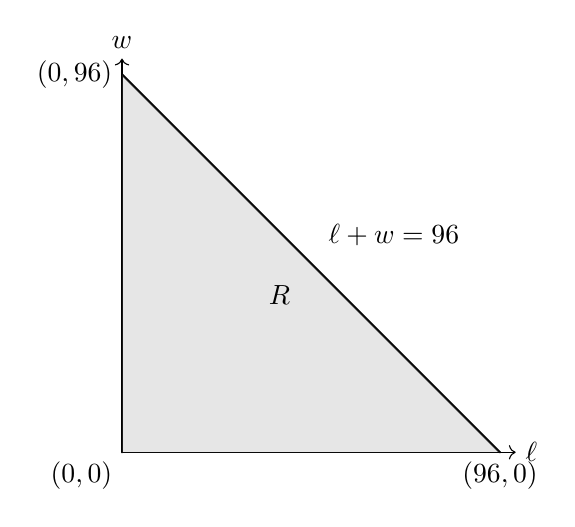
\begin{tikzpicture}[scale=0.05]
			% Draw the axes
			\draw[->] (0, 0) -- (100, 0) node[right] {\( \ell \)};
			\draw[->] (0, 0) -- (0, 100) node[above] {\( w \)};

			% Draw the boundary line l + w = 96
			\draw[thick] (0,96) -- (96,0);
			\node[above right] at (50, 50) {\( \ell + w = 96 \)};

			% Label points
			\filldraw[black] (96,0) circle (1.5pt) node[below] {\( (96, 0) \)};
			\filldraw[black] (0,96) circle (1.5pt) node[left] {\( (0, 96) \)};
			\filldraw[black] (0,0) circle (1.5pt) node[below left] {\( (0, 0) \)};

			% Shade the feasible region
			\fill[gray, opacity=0.2] (0, 0) -- (0, 96) -- (96, 0) -- cycle;

			% Label the region
			\node at (40, 40) {\( R \)};
		\end{tikzpicture}
	\end{center}

	Solving this, we find that \( V(32, 32) = 32 \cdot 32 \cdot 32 = 32768 \), which is the maximum value on \( R \).\\

	To confirm the local maximum at \( (32, 32) \), we compute the Hessian:
	\[
		H(\ell, w) = \begin{bmatrix} -2w & 96 - \ell - w \\ 96 - \ell - w & -2\ell \end{bmatrix}
	\]
	At \( (32, 32) \), the Hessian determinant is:
	\[
		\det(H) = (-2 \times 32)^2 - (96 - 32 - 32)^2 = (64 \times 64) - (32 \times 32) = 32768 > 0
	\]
	Thus, \( V(\ell, w) \) has a local maximum at \( (32, 32) \).
}
\ex{Another Example}{
	Consider \( f(x, y) = 4 - x^2 - y^2 \) on \( R = \{ (x, y) \mid -1 \leq x \leq 1, x^2 + y^2 < 1 \} \). Here, \( R \) is an open region without boundaries.\\

	The maximum of \( f(x, y) \) occurs at \( (0, 0) \), where \( f(0, 0) = 4 \). There is no absolute minimum because for points approaching the boundary (e.g., \( x \approx 0.99 \)), \( f(x, y) \) approaches \( -\infty \).

	Thus, in \( R \), there is no absolute minimum value for \( f \), illustrating the importance of the region's closedness and boundedness for the Extreme Value Theorem to apply.
}

\section{Lagrange Multiplier Method}

\subsection{General Procedure}

To maximize or minimize \( f(x, y) \) subject to a constraint \( g(x, y) = 0 \), follow these steps:

\begin{enumerate}
	\item \textbf{Identify Critical Points:} A point \( (x', y') \) is a critical point if:
	      \begin{itemize}
		      \item There exists \( \lambda \in \mathbb{R} \) such that \( \nabla f(x', y') = \lambda \nabla g(x', y') \) (using the \emph{method of Lagrange multipliers}).
		      \item \( g(x', y') = 0 \).
	      \end{itemize}

	\item \textbf{Evaluate Cases for Critical Points:}
	      \begin{enumerate}
		      \item \textbf{Case 1:} The constraint region \( R \) is bounded and has no endpoints.
		            \begin{itemize}
			            \item In this case, assuming continuity of \( f \), any local extrema within \( R \) are also absolute extrema.
			            \item Select critical points \( (x', y') \) and evaluate \( f \) at these points.
		            \end{itemize}

		      \item \textbf{Case 2:} The constraint region \( R \) is bounded and has endpoints.
		            \begin{itemize}
			            \item Example: \( x^2 - 4y^2 \leq 0 \) with \( -1 \leq x \leq 1 \).
			            \item Absolute extrema may occur at local extrema or endpoints.
			            \item Check critical points and also evaluate \( f \) at the boundary endpoints.
		            \end{itemize}

		      \item \textbf{Case 3:} The constraint region \( R \) is unbounded or does not include all endpoints.
		            \begin{itemize}
			            \item Example: \( x^2 - 4y^2 \) unbounded or \( x^2 + y^2 - 4 = 0 \) with \( -2 \leq x \leq 2 \).
			            \item It may be possible that absolute extrema do not exist.
			            \item Find any critical points and evaluate \( f(x) \) as \( x \rightarrow \pm \infty \) if applicable.
		            \end{itemize}
	      \end{enumerate}
\end{enumerate}

\ex{Lagrange Multiplier Method}{
	We aim to find the absolute extrema of the function \( f(x, y) = x - 2y \) subject to the constraint \( g(x, y) = x^2 + y^2 = 4 \).\\
	To find the extrema, we use the method of Lagrange multipliers, where we seek points where \( \nabla f = \lambda \nabla g \).

	The gradients of \( f \) and \( g \) are:
	\[
		\nabla f(x, y) = \begin{bmatrix} 1 \\ -2 \end{bmatrix}, \quad \nabla g(x, y) = \begin{bmatrix} 2x \\ 2y \end{bmatrix}
	\]
	Setting \( \nabla f = \lambda \nabla g \), we have:
	\[
		\begin{cases}
			1 = \lambda \cdot 2x \\
			-2 = \lambda \cdot 2y
		\end{cases}
	\]
	This simplifies to:
	\[
		\lambda = \frac{1}{2x} = \frac{-1}{y} \Rightarrow y = -2x
	\]

	Substitute \( y = -2x \) into the constraint \( g(x, y) = x^2 + y^2 = 4 \):
	\[
		x^2 + (-2x)^2 = 4 \Rightarrow x^2 + 4x^2 = 4 \Rightarrow 5x^2 = 4 \Rightarrow x = \pm \frac{2}{\sqrt{5}}
	\]
	Then, \( y = -2x \) gives \( y = \pm \frac{4}{\sqrt{5}} \). So the points are:
	\[
		\left( \frac{2}{\sqrt{5}}, -\frac{4}{\sqrt{5}} \right) \quad \text{and} \quad \left( -\frac{2}{\sqrt{5}}, \frac{4}{\sqrt{5}} \right)
	\]

	Calculate \( f(x, y) \) at the points:
	\[
		f\left( \frac{2}{\sqrt{5}}, -\frac{4}{\sqrt{5}} \right) = \frac{2}{\sqrt{5}} + \frac{8}{\sqrt{5}} = \frac{10}{\sqrt{5}} = 2\sqrt{5}
	\]
	\[
		f\left( -\frac{2}{\sqrt{5}}, \frac{4}{\sqrt{5}} \right) = -\frac{2}{\sqrt{5}} - \frac{8}{\sqrt{5}} = -\frac{10}{\sqrt{5}} = -2\sqrt{5}
	\]
	Thus, the \textbf{absolute maximum} is \( 2\sqrt{5} \) and the \textbf{absolute minimum} is \( -2\sqrt{5} \).\\

	Below is a diagram showing the constraint \( x^2 + y^2 = 4 \) as a circle and the level curves of \( f(x, y) = x - 2y \), specifically showing the two tangent level curves at \( z = \pm \frac{10}{\sqrt{5}} \) that represent the maximum and minimum values.

	\begin{center}
		\begin{tikzpicture}[scale=1.5]
			% Draw the constraint circle x^2 + y^2 = 4
			\draw[thick] (0,0) circle (2);
			\node at (2.2, 0) {\( x^2 + y^2 = 4 \)};

			% Draw the level curves of f(x, y) = x - 2y
			\draw[dashed, domain=-2:2] plot({\x}, {(\x - 10/sqrt(5))/2});
			\node[above right] at (1.788854382, -2) {\( x - 2y = \frac{10}{\sqrt{5}} \)};

			\draw[dashed, domain=-2:2] plot({\x}, {(\x + 10/sqrt(5))/2});
			\node[below right] at (1.788854382, 2) {\( x - 2y = -\frac{10}{\sqrt{5}} \)};

			% Draw the points of maximum and minimum
			\filldraw[black] (0.894427191, -1.788854382) circle (0.05);
			\node[below right] at (0.894427191, -1.788854382) {\( \left( \frac{2}{\sqrt{5}}, -\frac{4}{\sqrt{5}} \right) \)};

			\filldraw[black] (-0.894427191, 1.788854382) circle (0.05);
			\node[above left] at (-0.894427191, 1.788854382) {\( \left( -\frac{2}{\sqrt{5}}, \frac{4}{\sqrt{5}} \right) \)};
		\end{tikzpicture}
	\end{center}
}

\ex{Example: Finding Extrema of \( f(x, y) = e^{x+y} \) with Constraint}{
	Consider maximizing or minimizing \( f(x, y) = e^{x+y} \) subject to the constraint \( g(x, y) = x^2 + xy + y^2 - 9 = 0 \).

	\begin{enumerate}
		\item Using the method of Lagrange multipliers, we set up the system:
		      \[
			      \nabla f(x, y) = \lambda \nabla g(x, y)
		      \]
		      which gives:
		      \[
			      \begin{cases}
				      e^{x+y} = \lambda (2x + y) \\
				      e^{x+y} = \lambda (x + 2y)
			      \end{cases}
		      \]

		\item Dividing the equations, we get:
		      \[
			      \frac{2x + y}{x + 2y} = 1 \Rightarrow x = y
		      \]
		\item Substitute \( x = y \) into the constraint \( x^2 + xy + y^2 = 9 \):
		      \[
			      x^2 + x^2 + x^2 = 9 \Rightarrow 3x^2 = 9 \Rightarrow x = \pm \sqrt{3}, \quad y = \pm \sqrt{3}
		      \]
		\item The critical points are \( ( \sqrt{3}, \sqrt{3} ) \) and \( ( -\sqrt{3}, -\sqrt{3} ) \).

		\item Evaluating \( f(x, y) \) at these points:
		      \[
			      f(\sqrt{3}, \sqrt{3}) = e^{2\sqrt{3}}, \quad f(-\sqrt{3}, -\sqrt{3}) = e^{-2\sqrt{3}}
		      \]

		\item Thus, the maximum value is \( e^{2\sqrt{3}} \) and the minimum value is \( e^{-2\sqrt{3}} \).
	\end{enumerate}
}

\ex{Example: Finding Extrema of \( f(x, y) = x - y \) with Constraint}{
	Consider the function \( f(x, y) = x - y \) with the constraint \( g(x, y) = x^2 + y^2 - 3 x y - 20 = 0 \).

	\begin{enumerate}
		\item The gradients are:
		      \[
			      \nabla f(x, y) = \begin{bmatrix} 1 \\ -1 \end{bmatrix}, \quad \nabla g(x, y) = \begin{bmatrix} 2x - 3y \\ 2y - 3x \end{bmatrix}
		      \]

		\item Set \( \nabla f = \lambda \nabla g \):
		      \[
			      \begin{cases}
				      1 = \lambda (2x - 3y) \\
				      -1 = \lambda (2y - 3x)
			      \end{cases}
		      \]

		\item Solving this system, we find critical points at \( (2, -2) \) and \( (-2, 2) \).

		\item Evaluating \( f(x, y) \) at these points:
		      \[
			      f(2, 1) = 1, \quad f(-2, -1) = -1
		      \]

		\item Therefore, the maximum value is \( 1 \) and the minimum value is \( -1 \).
	\end{enumerate}

	By observing the level curves diagram, we can see that the given points do not maximise/minimise the function, as any other line where \( x-y < \pm 4 \) would further increase/decrease the function.

}

\begin{center}
	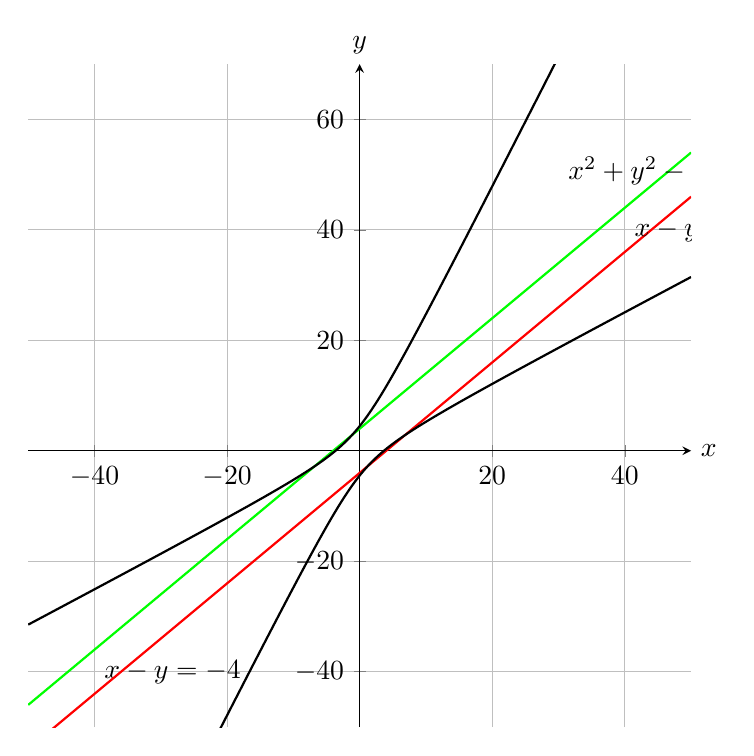
\begin{tikzpicture}
		\begin{axis}[
				axis lines=middle,
				grid=both,
				xmin=-50, xmax=50,
				ymin=-50, ymax=70,
				xlabel={$x$},
				ylabel={$y$},
				every axis x label/.style={at={(current axis.right of origin)}, anchor=west},
				every axis y label/.style={at={(current axis.above origin)}, anchor=south},
				width=10cm, height=10cm,
				samples=200,
				domain=-50:50
			]

			% Plot of x - y = -4
			\addplot[domain=-50:50, green, thick] {x + 4};
			\node[anchor=south west] at (axis cs:-40,-44) {$x - y = -4$};

			% Plot of x - y = 4
			\addplot[domain=-50:50, red, thick] {x - 4};
			\node[anchor=south west] at (axis cs:40,36) {$x - y = 4$};

			% Approximate implicit plot for x^2 + y^2 - 3xy - 20 = 0 using parametric plot
			\addplot[black, thick, samples=200, domain=-50:50] 
				({x}, {(3*x + sqrt(3*x*x + 80))/2});
			\addplot[black, thick, samples=200, domain=-50:50] 
				({x}, {(3*x - sqrt(3*x*x + 80))/2});
			\node[anchor=north west] at (axis cs:30,55) {$x^2 + y^2 - 3xy - 20 = 0$};

		\end{axis}
	\end{tikzpicture}
\end{center}


\section{Multiple Integration}

\nt{
	The integral
	\[
		\int_a^b f(x) \, dx = A
	\]
	represents the area under the curve \( f(x) \) from \( a \) to \( b \), where \( A \) can also be approximated as
	\[
		A \approx \sum_{i=1}^N f(x_i) \Delta x.
	\]
}

\nt{
To find the volume under a surface \( z = f(x, y) \) over a region \( R = [a, b] \times [c, d] \), we use the double integral
\[
	\iint_R f(x, y) \, dA.
\]
This can be approximated by summing over small subregions within \( R \):
\[
	\iint_R f(x, y) \, dA = \lim_{\Delta \to 0} \sum_{i=1}^m \sum_{j=1}^n f(x_i, y_j) \Delta x \, \Delta y.
\]
}

\thm{Continuity and Limits of Double Integrals}{
	If the limit
	\[
		\lim_{(x, y) \to (a, b)} f(x, y)
	\]
	exists for all points \( (a, b) \) in \( R \), then \( f(x, y) \) is continuous over \( R \), and the order of integration can be changed under Fubini's theorem.
}

\nt{
	Consider dividing \( R \) into \( n \) subregions, each with area \( \Delta A_{ij} \) and height \( f(x_i, y_j) \). Then, the volume \( V \) is approximated as
	\[
		V \approx \sum_{i=1}^m \sum_{j=1}^n f(x_i, y_j) \Delta x \, \Delta y,
	\]
	where \( n \) is the number of boxes in the \( x \)-direction and \( m \) is the number in the \( y \)-direction. Taking the limit as \( \Delta x, \Delta y \to 0 \) gives
	\[
		V = \iint_R f(x, y) \, dA.
	\]
}

\dfn{Double Integral Definition}{
The double integral of \( f(x, y) \) over \( R = [a, b] \times [c, d] \) is defined by
\[
	\iint_R f(x, y) \, dA = \lim_{n \to \infty} \sum_{i=1}^n \sum_{j=1}^n f(x_i, y_j) \Delta A_{ij}.
\]
}

\thm{Fubini's Theorem}{
	The order of integration does not affect the result of the double integral. Thus,
	\[
		\iint_R f(x, y) \, dA = \int_a^b \left( \int_c^d f(x, y) \, dy \right) dx = \int_c^d \left( \int_a^b f(x, y) \, dx \right) dy.
	\]
}

\ex{Example of Double Integral Calculation}{
Calculate the volume under \( f(x, y) = 4 + x + y^2 \) over the region \( R = [-1, 1] \times [0, 2] \):
\[
	\iint_R f(x, y) \, dA = \int_{-1}^1 \int_0^2 (4 + x + y^2) \, dy \, dx.
\]
Evaluating the inner integral with respect to \( y \),
\[
	\int_0^2 (4 + x + y^2) \, dy = 4y + xy + \frac{y^3}{3} \Big|_0^2 = 8 + 2x + \frac{8}{3}.
\]
Then, integrating with respect to \( x \),
\[
	\int_{-1}^1 \left( 8 + 2x + \frac{8}{3} \right) dx = \left( 8 + \frac{8}{3} \right) \cdot 2 = \frac{32}{3}.
\]
Thus, the volume \( V = \frac{32}{3} \).
}

\ex{Example: Integration Over a Rectangular Domain}{
	Evaluate
	\[
		\int_0^2 \int_0^1 \frac{x y}{1 + x^2} \, dx \, dy.
	\]

	Using substitution \( u = x^2 \) with \( du = 2x \, dx \), we find
	\[
		\int_0^2 \int_0^1 \frac{x y}{1 + x^2} \, dx \, dy = \int_0^2 y \left( \int_0^1 \frac{x}{1 + x^2} \, dx \right) dy = \int_0^2 y \left[ \frac{1}{2} \ln(1 + x^2) \right]_0^1 \, dy.
	\]
	Simplifying, we get
	\[
		V = \int_0^2 y \cdot \frac{\ln(2)}{2} \, dy = \frac{\ln(2)}{2} \int_0^2 y \, dy = \frac{\ln(2)}{2} \cdot \frac{y^2}{2} \Big|_0^2 = \ln(2).
	\]
}

\subsection{Non-Rectangular Domains}

\nt{
	Consider \( R = \{ (x, y) : a \leq x \leq b, g_1(x) \leq y \leq g_2(x) \} \), where the boundaries are given by functions \( y = g_1(x) \) and \( y = g_2(x) \).
}

\ex{Example: Non-Rectangular Domain Integration}{
	Suppose \( R = \{ (x, y) : -1 \leq x \leq 1, x^2 \leq y \leq 2 - x^2 \} \).
	We wish to evaluate
	\[
		\int_R (x+y) \, dA.
	\]
	We split \( R \) into two regions, \( R_1 \) and \( R_2 \), with bounds given by
	\[
		R_1 = \{ (x, y) : -1 \leq x \leq 1, x^2 \leq y \leq 2 - x^2 \}.
	\]
	Evaluating each integral, we obtain
	\[
		V = \int_{-1}^1 \left( \int_{x^2}^{2 - x^2} (x + y) \, dy \right) dx.
	\]

	On solving, we get
	\[
		V = \int_{-1}^1 \left( \int_{x^2}^{2 - x^2} (x + y) \, dy \right) dx = \ldots = \frac{8}{35}.
	\]
}

\begin{center}
	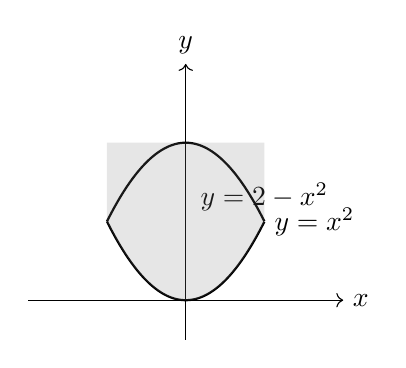
\begin{tikzpicture}
		% Define axes
		\draw[->] (-2,0) -- (2,0) node[right] {\( x \)};
		\draw[->] (0,-0.5) -- (0,3) node[above] {\( y \)};

		% Draw the curves
		\draw[thick, domain=-1:1, samples=100] plot (\x, {\x*\x}) node[right] {\( y = x^2 \)};
		\draw[thick, domain=-1:1, samples=100] plot (\x, {2 - \x*\x}) node[above] {\( y = 2 - x^2 \)};

		% Shade the region between curves
		\fill[gray, opacity=0.2] (-1,1) parabola bend (0,0) (1,1) -- (1,2) parabola bend (0,2) (-1,2) -- cycle;
	\end{tikzpicture}
\end{center}

\nt{
	When changing the order of integration, try dividing the region into smaller regions to make integration simpler.
}

\subsection{Volume Between Surfaces}

\nt{
	To find the volume of a sphere using double integrals, consider the surface
	\[
		x^2 + y^2 + z^2 = 1.
	\]
	Then \( z = \pm \sqrt{1 - x^2 - y^2} \), and we can set up the integral as
	\[
		V = 2 \iint_R \sqrt{1 - x^2 - y^2} \, dA,
	\]
	where \( R = \{ (x, y) : -1 \leq x \leq 1, -\sqrt{1 - x^2} \leq y \leq \sqrt{1 - x^2} \} \).
}

\begin{center}
	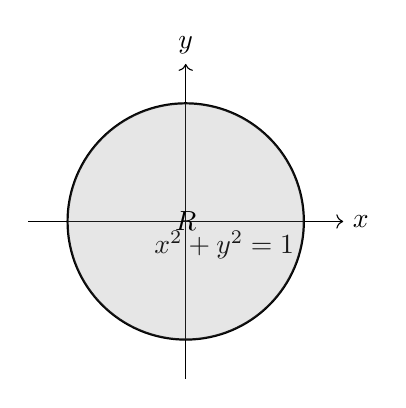
\begin{tikzpicture}
		% Define axes
		\draw[->] (-2,0) -- (2,0) node[right] {\( x \)};
		\draw[->] (0,-2) -- (0,2) node[above] {\( y \)};

		% Draw the circle for the sphere projection
		\draw[thick] (0,0) circle (1.5);
		\node[below left] at (1.5,0) {\( x^2 + y^2 = 1 \)};

		% Label the region
		\fill[gray, opacity=0.2] (0,0) circle (1.5);
		\node at (0,0) {\( R \)};
	\end{tikzpicture}
\end{center}

\ex{Example: Volume Between Surfaces}{
	Calculate the volume between the surfaces \( z = \sqrt{1 - x^2 - y^2} \) and \( z = -\sqrt{1 - x^2 - y^2} \):
	\[
		V = \iint_R \left( \sqrt{1 - x^2 - y^2} - (-\sqrt{1 - x^2 - y^2}) \right) \, dA = 2 \iint_R \sqrt{1 - x^2 - y^2} \, dA.
	\]
	Setting up the limits as before, we integrate over \( R \) to find the volume of the sphere.
}

\end{document}